% begin module curve-sketching-guidelines
\begin{frame}
\frametitle{Guidelines for Sketching a Curve}
The following items are to be considered when drawing a curve. \alert<2>{Not every item is relevant to every function.}
\begin{enumerate}
\item  Determine the domain of the function.
\item  Depending on availability, use computer software to plot. 
\item  \alert<2>{Compute $x,y$ intercepts.}
\item  \alert<2>{Determine symmetries, periodicity.}
\item  \alert<2>{Compute asymptotes - vertical, horizontal, {\color{gray} optional - slanted}.}
\item  Compute intervals of increase or decrease.
\item  Compute local and global maxima and minima.
\item  Compute concavity and points of inflection.
%\item  Sketch the curve
\end{enumerate}
\end{frame}

\begin{frame}[t]
\begin{enumerate}
\item  \alert<3>{Domain}
\begin{itemize}
\item  Find the domain of the function.  
\item  Remember the two restrictions: no dividing by $0$, and no taking the even root of a negative number.
\end{itemize}
\item<2-> You can use computer software to plot your function.
\begin{itemize}
\item<3-> Most computer software will ask you to specify the \alert<3>{domain of the function} explicitly.
\item<4-> Some software may be able to determine the (implied) domain of your function.
\item<5-> Software may not be always available (example: Calculus I exams).
\end{itemize} 
\end{enumerate}
\end{frame}


\begin{frame}[t]
\begin{enumerate}
\setcounter{enumi}{2}
\item  Intercepts
\end{enumerate}
\begin{itemize}
\item  Find the intercepts of the function.
\item  $f(0)$ is the $y$-intercept.
\item  To find the $x$-intercepts, set $y = 0$ and solve for $x$.
\item  You can sometimes skip this step if the equation is too difficult to solve.
\end{itemize}
\end{frame}


\begin{frame}[t]
\begin{enumerate}
\setcounter{enumi}{3}
\item  Symmetry, Periodicity
\end{enumerate}
\begin{itemize}
\item<1-| alert@2>  \alert<handout:1| 0>{If $f(-x) = f(x)$ for all $x$, then $f$ is even.}
\item<1-| alert@3>  \alert<handout:2| 0>{If $f(-x) = -f(x)$ for all $x$, then $f$ is odd.}
\item<1-| alert@4>  \alert<handout:3| 0>{If there is some number $p$ such that $f(a+p) = f(a)$ for all $a$, then $f$ is called periodic.  The smallest such $p$ is called its period.}
\end{itemize}
\begin{center}

\ \only<handout:1| -2>{%
\uncover<2>{%
\psset{xunit=1cm, yunit=1cm}
\begin{pspicture}(-1.7, -5)(1.7,5) 
\psframe*[linecolor=white](-1.7,-5)(1.7,5) 
\tiny 
\psaxes[ticks=none, labels=none]{<->}(0,0)(-1.7,-1.5)(1.7,2.5721)
\psLabels{1.7}{2.5721}
\psXTickWithLabel{-1}{$-1$}
\psXTickWithLabel{1}{$1$}
%Function formula: -2 x^{2}+x^{4} 
%\rput(1,3){$y=-2 x^{2}+x^{4}$} 
\psFullDot{-1.5}{0.5625}
\psFullDot{1.5}{0.5625}
\rput[r](-1.6, 0.5625){$(-1.5, f(1.5))$}
\rput[l](1.6, 0.5625){$(1.5, f(1.5))$}
\psline{<->}(-1.4, 0.5625)(1.4, 0.5625)
\psFullDot{-1}{-1}
\psFullDot{1}{-1}
\rput[rt](-1.1, -1){$(-1, f(1))$}
\rput[lt](1.1, -1){$(1, f(1))$}
\psline{<->}(-0.9, -1)(0.9, -1)

\psplot[linecolor=\psColorGraph, plotpoints=1000]{-1.7}{1.7}{x 4 exp x 2 exp -2 mul add }
\end{pspicture}
}}%
\only<handout:2| 3>{%
\psset{xunit=1cm, yunit=1cm}
\begin{pspicture}(-3, -5)(3,5) 
\psframe*[linecolor=white](-3,-5)(3,5) 
\tiny 
\psaxes[ticks=none, labels=none]{<->}(0,0)(-3.2,-2)(3.2,2)
\psLabels{3.2}{2}
\psXTickWithLabel{1}{$1$}
\psXTickWithLabel{-1}{$-1$}
%Function formula: \sin{}x 
\psplot[linecolor=\psColorGraph, plotpoints=1000]{-3}{3}{x 57.29578 mul sin }
%Function formula: \sqrt{- x^{2}+17080660249/10000000000} 
\psplot[arrows=->, plotpoints=1000]{-1.3068}{0.92}{1.70807 x 2 exp -1 mul add sqrt }
%Function formula: -\sqrt{- x^{2}+17080660249/10000000000} 
\psplot[arrows=->, plotpoints=1000]{-1.3068}{-1.08}{1.70807 x 2 exp -1 mul add sqrt -1 mul}
\psFullDot{1}{0.841471}
\rput[lt](1,0.741471 ){$(1, f(1))$}
\psFullDot{-1}{-0.841471}
\rput[t](-1,-1.05 ){$(-1, -f(1))$}
\rput[lb](1.5, 1.1){$y=f(x)$}
\end{pspicture}
}%

\only<handout:3| 4->{%
\psset{xunit=0.8cm, yunit=0.8cm}
\begin{pspicture}(-10, -5)(10,5) 
\psframe*[linecolor=white](-10,-5)(10,5) 
\tiny 
\psaxes[ticks=none, labels=none]{<->}(0,0)(-6,-0.7)(6,4.5)
\psLabels{6}{4.5}
%Function formula: \sin^{2}{}(2 x)+\sin{}(2 x)+1 
%\rput(1,3){$y=\sin^{2}{}(2 x)+\sin{}(2 x)+1$} 
\psplot[linecolor=\psColorGraph, plotpoints=1000]{-6}{6}{1 x 2 mul 57.29578 mul sin add x 2 mul 57.29578 mul sin 2 exp add }

\psFullDot{0.785398163}{3}
\psline[linestyle=dashed](0.785398163,0)(0.785398163,3)
\psXTickWithLabel{0.785398163}{$a+p$}
\psFullDot{3.926990817}{3}
\psline[linestyle=dashed](3.926990817,0)(3.926990817,3)
\psXTickWithLabel{3.926990817}{$a+2p$}
\psFullDot{-2.35619449}{3}
\psline[linestyle=dashed](-2.35619449,0)(-2.35619449,3)
\psXTickWithLabel{-2.35619449}{$a$}
\psFullDot{-5.497787144}{3}
\psline[linestyle=dashed](-5.497787144,0)(-5.497787144,3)
\psXTickWithLabel{-5.497787144}{$a-p$}

\end{pspicture} 
}

%\ \only<handout:1| -2>{%
%\uncover<2>{%
%\ 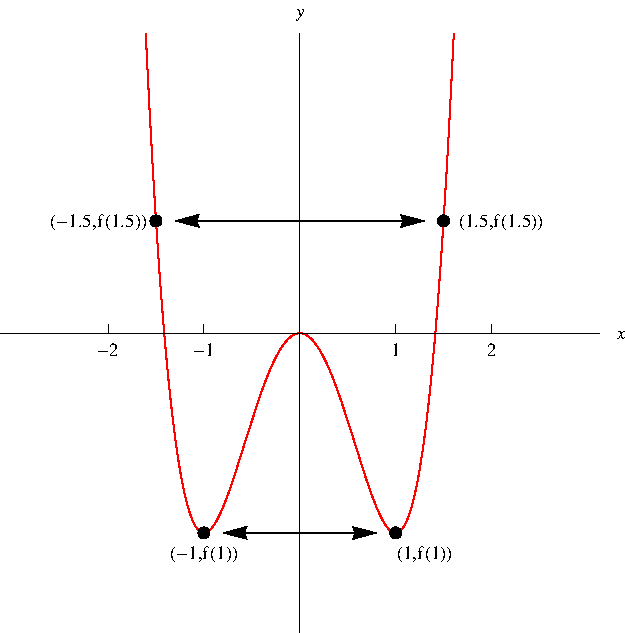
\includegraphics[height=5cm]{curve-sketching/pictures/01-01-even.pdf}%
%}}%
%\only<handout:2| 3>{%
%\ 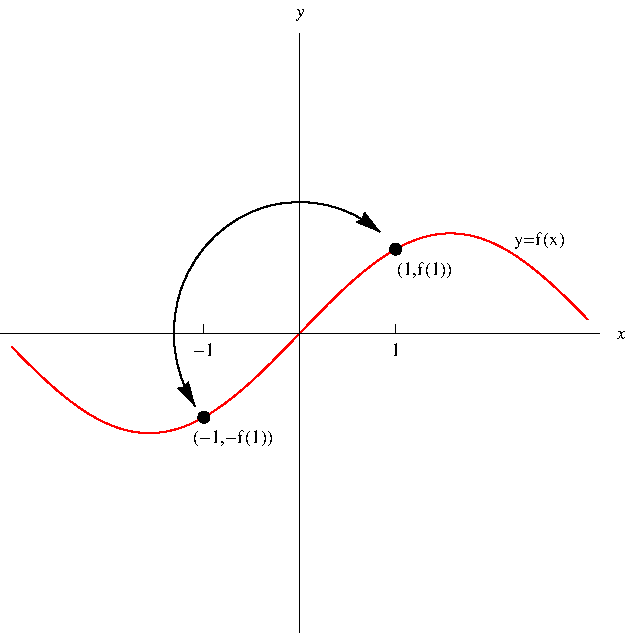
\includegraphics[height=5cm]{curve-sketching/pictures/01-01-odd.pdf}%
%}%
%\only<handout:3| 4->{%
%\ 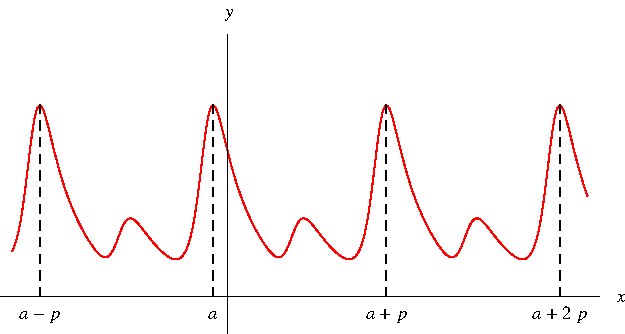
\includegraphics[height=5cm]{curve-sketching/pictures/04-05-periodic.pdf}%
%}
\end{center}
\end{frame}


\begin{frame}[t]
\begin{enumerate}
\setcounter{enumi}{4}
\item  Asymptotes
\end{enumerate}
\begin{itemize}
\item  \textbf{Horizontal asymptotes} can be found by finding $\lim_{x\to\infty} f(x)$ and $\lim_{x\to -\infty} f(x)$.
\item  If either of these equals a number $L$, then $y = L$ is a horizontal asymptote of $f$.  
\item  If neither limit is finite, there is no horizontal asymptote.
\item  The line $x = a$ is a \textbf{Vertical asymptote} of $f$ if any of the following is true
\end{itemize}
\[
\begin{array}{ll}
\displaystyle \lim_{x\to a^+}f(x) = \infty &%
\displaystyle \lim_{x\to a^-}f(x) = \infty \\%
\displaystyle \lim_{x\to a^+}f(x) = -\infty &%
\displaystyle \lim_{x\to a^-}f(x) = -\infty %
\end{array}
\]
\begin{itemize}
\item  We will discuss \textbf{slant asymptotes} later in section 4.5.
\end{itemize}
\end{frame}


\begin{frame}[t]
\begin{enumerate}
\setcounter{enumi}{5}
\item  Intervals of increase or decrease
\end{enumerate}
\begin{itemize}
\item  To find intervals of increase or decrease, use the increasing/decreasing test.
\item  Compute $f'$.
\item  Find where $f'$ is positive or negative.
\item  Where $f'$ is positive, $f$ is increasing.
\item  Where $f'$ is negative, $f$ is decreasing.
\end{itemize}
\end{frame}




\begin{frame}[t]
\begin{enumerate}
\setcounter{enumi}{6}
\item  Local maxima and minima
\end{enumerate}
\begin{itemize}
\item  Find the critical numbers of $f$ (the numbers $c$ where $f'(c)$ doesn't exist or $f'(c) = 0$).
\item  Use the First Derivative Test on each of these numbers:
\item  If $f'$ changes from positive to negative at a critical number $c$, then $c$ is a local maximum.
\item  If $f'$ changes from negative to positive at a critical number $c$, then $c$ is a local minimum.
\item  If $f'$ doesn't change sign at a critical number $c$, then $c$ is neither a local maximum nor a local minimum.
\end{itemize}
\end{frame}



\begin{frame}[t]
\begin{enumerate}
\setcounter{enumi}{7}
\item  Concavity and points of inflection
\end{enumerate}
\begin{itemize}
\item  To find inflection points and intervals of concavity, use the concavity test.
\item  Compute $f''$.
\item  Find where $f''$ is positive or negative.
\item  Where $f''$ is positive, $f$ is concave up.
\item  Where $f''$ is negative, $f$ is concave down.
\item  Inflection points occur when $f''$ changes signs.
\end{itemize}
\end{frame}
% end module curve-sketching-guidelines
